\documentclass[11pt,a4paper]{article}

% Core packages
\usepackage[utf8]{inputenc}
\usepackage[T1]{fontenc}
\usepackage{lmodern}
\usepackage{microtype}
\usepackage[margin=1in]{geometry}

% Bibliography
\usepackage[numbers,sort&compress]{natbib}

% Figures and tables
\usepackage{graphicx}
\usepackage{booktabs}
\usepackage{longtable}
\usepackage{array}
\usepackage{multirow}

% TikZ
\usepackage{tikz}
\usepackage{pgfplots}
\pgfplotsset{compat=1.18}
\usetikzlibrary{arrows.meta,positioning,shapes.geometric,fit,backgrounds,calc}

% Math
\usepackage{amsmath,amssymb,amsthm}

% Links
\usepackage[colorlinks=true,linkcolor=blue,citecolor=blue,urlcolor=blue]{hyperref}

% Headers
\usepackage{fancyhdr}
\pagestyle{fancy}
\fancyhf{}
\rhead{\thepage}
\setlength{\headheight}{14pt}

%% -----------------------------------------------------------------------
%% PAPER METADATA -- fill in before compiling
%% -----------------------------------------------------------------------
\title{Start Fast, Stop Fast: Interruptibility and the Cessation Floor of\\ Realtime Cascade Voice Agents}

% Author block (manual; no authblk dependency)
\author{Daniel Garc\'ia Pe\~na\\
  \small Department of Energy and Process Control, University of Oviedo, Oviedo, Spain.\\
  \small AI Engineering, Unicaja Bank, Spain.
  \texttt{info@iamdgarcia.com}}

\date{\today}

%% Theorem environments (mirror the companion latency-floor paper)
\newtheorem{definition}{Definition}
\newtheorem{theorem}{Theorem}
\newtheorem{lemma}[theorem]{Lemma}
\newtheorem{corollary}[theorem]{Corollary}
\newtheorem{proposition}[theorem]{Proposition}
\theoremstyle{definition}
\newtheorem{example}{Example}
\newtheorem{remark}{Remark}

\begin{document}

\maketitle

\begin{abstract}
Perceived responsiveness of a realtime cascade voice agent has two floors: response \emph{onset}
(how fast the agent can first be heard) and response \emph{cessation} (how fast it fully stops
when the user interrupts). The onset floor is well characterised; the cessation floor is neither
standardly defined nor formally bounded. We introduce the two-floor model, prove a
phase-conditioned cessation floor (detect/decide/cease/resume) that grows with in-flight audio
$\approx$ queue depth $\times$ frame, and show how tool round-trips sit on the onset side unless
dispatched to a background execution clock. A new API-serializability lemma makes tool persistence
under cancellation safe: an interrupted turn cancels generation while pending tool batches commit
atomically. We argue decoupled-clocks (event-driven) scheduling is the idiomatic configuration
that owns both floors, validate the semantics with a small tested orchestrator, and anchor the
quantitative claims with a monotonic-clock smoke measurement: cessation is linear in in-flight
audio ($109$~ms at buffer depth 1 vs $609$~ms at depth 6), generation cancellation is prompt
and depth-independent, and resume after interruption is dominated by tool round-trip cost
($<$1~ms in-memory vs $\sim$1~s remote).
Together the two floors give a complete, stage-level account of perceived responsiveness for
cascade agents, extending the onset-side guarantee to the orchestration that schedules
reasoning, tools, and interruption handling.
\end{abstract}

\section{Introduction}
\label{sec:introduction}
% §1 Introduction
Voice-based conversational agents are no longer a laboratory curiosity: they answer
telephone calls, operate bank accounts, and route service requests on a daily basis
\citep{openai2024realtimeapi,google2024geminivoice}.
Two architectural families dominate this space.
\emph{Native voice models} process speech end-to-end inside a single network, eliminating
inter-component boundaries and their latencies \citep{defossez2024moshi}.
\emph{Cascade architectures} decompose the agent into speech recognition, a text-based
language model, and speech synthesis, exposing transcripts and structured outputs that make
tool use, debugging, and governance practical \citep{yao2023react,langgraph2024}.
Modern cascades are valued precisely because they compose commodity components, swap
models independently, and call external tooling and databases mid-conversation.

The price of the cascade is latency.
Perceptual studies converge on a turn-taking norm of roughly $200$~ms
\citep{levinson2015timing,stivers2009universals}: responses slower than this are perceived as
delayed.
Our companion paper \citep{latencyfloor2025} formalises the \emph{onset} side of responsiveness for cascades: the
Latency Floor Theorem states that the silence gap from end of user speech to first audible
agent audio has an irreducible lower bound, and the Cascade Competitiveness Criterion states
when a cascade can meet the $200$~ms norm.
That work leaves the pipeline's middle stage as a black box and, crucially, addresses only
\textbf{when the agent starts to speak}.

Responsiveness has a second, equally visible half: \textbf{when the agent can fully stop}.
A user who interrupts a banking agent to correct an account number experiences, in that
instant, how much sound the agent keeps making and how long before the system is again
listening.
On tool-heavy turns this stopping behaviour dominates the felt quality of the assistant.
Yet the cessation side is neither standardly defined nor formally bounded: the turn-taking
literature treats barge-in operationally \citep{raux2008optimizing,skantze2021turn}, and
engineers measure barge-in behaviour ad hoc without a shared definition or a lower bound.

This paper supplies the missing floor.
We introduce a two-floor model of realtime responsiveness, prove a phase-conditioned
\emph{cessation floor} for cascade agents, and show how tool round-trips couple to the onset
floor unless they are scheduled onto a background execution clock.
We prove an API-serializability lemma that makes \emph{tool persistence under cancellation}
safe: an interrupted turn cancels generation while pending tool batches commit atomically.
We argue that decoupled-clocks (event-driven) scheduling is the idiomatic configuration that
owns both floors — a sufficiency claim, not a uniqueness claim.
We validate the required semantics with a small, tested, event-driven orchestrator and anchor
the quantitative statements with a monotonic-clock smoke measurement.

Our contributions are:
\begin{enumerate}
  \item a two-floor model of responsiveness (onset floor from our companion work
        \citep{latencyfloor2025}, cessation floor introduced here), together with
        Proposition~\ref{prop:floor_dependency} stating the dependency structure between the
        floors;
  \item a phase-conditioned cessation floor (generate / playback / tool-wait) with a
        detect--decide--cease--resume decomposition and separated \emph{can stop}
        (physical) and \emph{should stop} (policy) statements
        (Theorem~\ref{thm:cessation_floor});
  \item a tool-hiding coupling result showing that tool round-trips sit on the onset side
        unless dispatched to a background execution clock (Theorem~\ref{thm:tool_hiding});
  \item an API-serializability lemma making tool persistence under cancellation safe
        (Lemma~\ref{lem:serializability}) and a filler-placement corollary
        (Corollary~\ref{cor:filler});
  \item a small, tested, event-driven orchestrator providing faithful semantics, plus a
        measured smoke anchor of the cessation floor.
\end{enumerate}

The rest of the paper is structured as follows.
Section~\ref{sec:background} positions the work against incremental dialogue processing,
endpointing, interruption, and orchestration literature.
Section~\ref{sec:framework} defines the two-floor framework and the event system.
Section~\ref{sec:analysis} states and proves the results.
Section~\ref{sec:practical} answers the practitioner's question of which cascade
architecture to build.
Section~\ref{sec:open_problems} lists open directions.
Section~\ref{sec:discussion} discusses scope and limitations, and
Section~\ref{sec:conclusion} concludes.


\section{Background and Related Work}
\label{sec:background}
% §2 Background and Related Work
\emph{References note:} all related-work references in this paper were verified against the
arXiv API and Crossref on 2026-09-01, including a 2025--26 sweep that surfaced the
full-duplex and interruption benchmark wave discussed in Section~\ref{sec:background} (\S2.7).

We position this paper against five bodies of work.
For each we state what it contributes and, explicitly, where it stops short of a formal
cessation floor.

\subsection{Incremental processing and revocable output}
The closest formal ancestor of a cessation floor is the incremental dialogue-processing
literature.
Schlangen and Skantze \citep{schlangen2011general} model dialogue systems as incrementally
communicating modules whose output units are produced left to right and can be revised or
cancelled.
Toolkits such as InproTK instantiate precisely this revocability for incremental speech
synthesis \citep{baumann2012prosodic}.
That line of work established that output increments are \emph{cancellable} behaviours, but it
was developed for pre-LLM statistical components, carries no agent-orchestration or
tool-execution semantics, and offers no lower-bound arithmetic for interruption reaction.
Our paper is exactly the missing latency-bound layer: it keeps revocability as the substrate
and asks how fast, per architecture, the agent can \emph{fully stop} while a tool waits.

\subsection{Endpointing, barge-in, and interruption policy}
Endpointing is the known latency-versus-reliability trade of detecting when the user stopped
talking: firing late adds silence to the onset floor, firing early risks cutting the user off
\citep{raux2008optimizing}.
Subsequent deployed work extracts the barge-in vs response-delay trade at scale
\citep{raux2012optimizing}.
Bohus and Horvitz \citep{bohus2011interruptions} go further and treat interruption as an
engagement \emph{decision}: sometimes the right behaviour is to keep talking, and deciding
whether to yield is policy, not physics.
These are the empirical and policy pillars our decomposition builds on.
Their gap is the same one: none states a lower bound on how long the agent's audio tail keeps
sounding after the user interrupts, nor how that bound depends on the architecture.

\subsection{Turn-taking timing and the two directions of responsiveness}
Human conversation shows modal gaps near $0$--$200$~ms with frequent sub-$100$~ms transitions
and ordered overlaps, not errors \citep{levinson2015timing,stivers2009universals,schegloff2000overlap}.
Quantitative corpus work further shows that a large share of transitions occur at or below
approximately $100$~ms, so a single threshold under-describes the distribution
\citep{heldner2010gaps}.
Backchannel placement is itself a timed behaviour: listeners tend to respond around a fixed
window after prosodic cues \citep{ward2000backchannel}.
Synthetic agents, for their part, lack a standard method for evaluating turn-taking behaviour
at all \citep{skantze2021turn}.
We use this literature to separate two responsiveness directions: producing one's first word
(onset) and releasing the floor (cessation), and we treat overlap as an orderly behaviour the
agent must be fast enough to support.

\subsection{Native full-duplex models}
End-to-end speech models such as Moshi demonstrate full-duplex dialogue with roughly $200$~ms of
streaming latency and visible interruption handling \citep{defossez2024moshi}, and commercial
APIs expose native speech-in/speech-out with built-in function calling
\citep{openai2024realtimeapi,google2024geminivoice}.
These systems are the architectural contrast for our per-topology cessation analysis: their
interruption reaction is bounded by codec-frame granularity, whereas a cascade's is bounded by
whatever audio is already in its synthesis queue.

\subsection{Agent orchestration, tools, and inference}
ReAct interleaves reasoning and tool acting \citep{yao2023react}, and graph frameworks such as
LangGraph make the resulting loops stateful and check-pointed \citep{langgraph2024}.
Chain-of-thought prompts make each reasoning step a visible latency component
\citep{wei2023chainofthought}.
Speculative decoding accelerates the reducible decode term without touching first-token or tool
delay \citep{leviathan2023fast}, and streaming long-context service is a serving-layer
concern \citep{xiao2023streamingllm}.
Finally, guardrail classification is increasingly placed inside the pipeline, where it must fit
a deadline rather than run after the fact \citep{dong2024building}.
This body of work motivates our setting: agents that reason, call tools, and are constrained by
a latency budget.
What it lacks is a formal treatment of \emph{interruptibility} as a schedulable property of
the orchestration rather than a property of any single component.

A separate line of engineering practice attacks tool latency directly: retrieval
round-trips are overlapped with drafting \citep{specrag2024}, intent prefetching lets an
assistant answer without a tool call at all \citep{agentsnotenough2024}, and the newest
full-duplex benchmarks evaluate tool use under streaming conditions
\citep{lin2026fdbv3}.
These are empirical existence proofs of the type-B/C hiding window we formalise in
Theorem~\ref{thm:tool_hiding}; none of them states a composition rule for when hiding is
possible or what unhideable type-A cost remains.
On the orchestration-operational side, graph frameworks already expose interrupt and
checkpoint primitives for human-in-the-loop reentry \citep{langgraph2024}; our point is that
such primitives are treated as operational features rather than as a schedulable latency
property.

\subsection{Recent full-duplex and interruption benchmarks}
A concurrent 2025--26 wave of benchmarks measures turn-taking and interruption behaviour
empirically.
Full-Duplex-Bench evaluates overlap handling in full-duplex spoken dialogue models
\citep{lin2025fullduplexbench}, its v3 extends this to tool use under streaming conditions
\citep{lin2026fdbv3}, and Easy Turn addresses turn-taking detection robustness
\citep{li2025easyturn}.
IHBench evaluates post-interruption recovery in structured-workflow voice agents
\citep{salimi2026ihbench}.
These works define and measure interruption and recovery \emph{outcomes} -- task success,
overlap accuracy, recovery outcome -- empirically.
None of them derives a formal lower bound on reaction latency per architecture (cascade vs
full-duplex vs decoupled), nor the phase-conditioned decomposition of the stop path.
The present paper supplies that missing formal account and is thus complementary to, not in
competition with, this benchmark wave.

\subsection{Position relative to the onset floor}
Our companion paper \citep{latencyfloor2025} bounds response onset for cascades and derives a
$k$-step silence-gap bound
for tool-using agents.
It treats the orchestration inside the language stage as a black box and stops at onset,
closing its open-problems discussion by explicitly flagging barge-in reaction as
untreated.
This paper opens that box: it bounds the other direction of responsiveness and shows that the
orchestrator's scheduling policy, not the components, decides whether reducible latency is
hidden or paid.
Its reactive cessation floor and the companion's predictive turn-end ceiling together delimit
the intervention window an agent can exploit.


\section{The Two-Floor Framework}
\label{sec:framework}
% §3 The Two-Floor Framework
We formalise responsiveness as two floors, model the orchestration that determines them, and
define the vocabulary used throughout the analysis.
All latency values refer to a fixed in-flight policy: a fixed endpointing configuration, a
fixed TTS buffer depth, and a fixed decode speed.

\begin{definition}[Responsiveness floors]
\label{def:floors}
For a single agent turn, \emph{response onset} is the interval from the detectable end of the
user's turn to the first audible unit of the agent's response.
\emph{Response cessation} is the interval from the first detectable onset of a user
interruption to the moment no further audibility of the agent's prior turn remains.
\end{definition}

Onset is the object of the companion Latency Floor Theorem and its Cascade Competitiveness
Criterion.
Cessation is the object of this paper.
The two intervals are disjoint in time but not in their dependencies: both read the same
detection subsystem, buffer policy, and decode speed.

\begin{definition}[Three clocks]
\label{def:clocks}
An orchestrator maintains three clocks over a turn.
The \emph{generation clock} tracks the language model's streamed output.
The \emph{delivery clock} tracks what has been handed to the speech synthesis and playback
path.
The \emph{tool clock} tracks tool execution scheduled in the background.
Control flow is expressed as events: a user turn, a tool completion, a delivery-started,
delivery-completed, or delivery-interrupted.
\end{definition}

The decoupling of the three clocks is the orchestration property under study.
A \emph{serial} topology couples all three clocks inside one call stack; a
\emph{concurrent} topology schedules them independently.

\begin{definition}[Interruption phases]
\label{def:phases}
An interruption lands in one of three phases of the agent's turn:
\emph{phase-gen} while generation runs but nothing is yet audible,
\emph{phase-play} while audio is being delivered, and
\emph{phase-tool} while the agent waits on a background tool.
\end{definition}

The phase determines what ``stopping'' means and which floor is re-entered afterwards.

\begin{definition}[Tool typing]
\label{def:tool_typing}
A tool is of
\emph{type A} if its result is required before any response audio can be produced,
\emph{type B} if its result can be deferred past the streaming-TTS lead-in, and
\emph{type C} if its result is needed only for a later turn.
\end{definition}

Type-A tools gate first audio and therefore sit on the onset floor; types B and C admit
hiding behind delivery lead-in or background execution.

\begin{definition}[Interruptibility]
\label{def:interruptibility}
An orchestrator is \emph{generation-interruptible} if cancelling the active model stream is a
first-class primitive.
It is \emph{execution-persistent} if cancelling generation does not cancel background tool
execution: pending tool calls continue, complete, and re-enter the model with their results.
\end{definition}

These two predicates jointly describe the capability that a cessation analysis operates on;
how \emph{fast} the capability is realised is set by the in-flight granularity of the
delivery and tool clocks.

\begin{definition}[API-valid history]
\label{def:apivalid}
A conversation history is \emph{API-valid} if it contains no assistant message whose tool-call
batch lacks its complete set of tool-result messages, for the model provider's function-calling
protocol.
\end{definition}

API-validity is the serializability constraint that tool persistence must respect: a pending
batch cannot be flushed to the provider, and cannot be abandoned without making the history
unplayable.

\subsection{An event system as the mechanism}
We instantiate the three clocks as an event-driven orchestrator: user texts and tool
completions are generic events; delivery status is reported back by the transport
(started, completed, interrupted); and interruption cancels the generation task without
touching the tool dispatcher.
Interrupted delivery is recorded and exposed as internal context on the next model
invocation, so the agent knows its previous response may not have been heard.
This instantiation is the object of the PoC validation in
Section~\ref{sec:analysis}; it is the configuration against which the serial topologies of
Section~\ref{sec:practical} are compared, not a uniqueness claim.


\section{Analysis: Ceasing and Hiding Latency}
\label{sec:analysis}
% §4 Analysis: Ceasing and Hiding Latency
We state and prove the two-floor results.
Throughout, $\Lambda_{on}$ and $\Lambda_c$ denote the onset and cessation floors of
Definition~\ref{def:floors}.
Constituent latencies of the pipeline are written $\lambda_{\cdot}$, with superscript $irr$
meaning \emph{irreducible}; reaction components of an interruption are written
$\delta_{\cdot}$ (\emph{detect}, \emph{decide}, \emph{cease}, \emph{resume}).
$\tau_f$ is the duration of one synthesis frame and $d$ the committed buffer depth of the
delivery clock.
By a ``floor'' we mean the infimum latency over admissible scheduler decisions under the fixed
in-flight policy of Definition~\ref{def:floors}.

\subsection{The dependency structure of the two floors}
We state the dependency relation as a proposition rather than a theorem: it is close to
definitional, but the shared subsystems are the load-bearing observation.

\begin{proposition}[Floor-constituent dependency]
\label{prop:floor_dependency}
Under a fixed in-flight policy (fixed detection configuration, buffer depth $d$, decode
speed), the onset floor and the cessation floor are set by largely disjoint pipeline
segments, except for three shared subsystems.
Writing $\lambda_s^{on}$ and $\lambda_s^{c}$ for the onset-side and cessation-side
contributions of a shared subsystem $s \in \{ \mathrm{detect}, \mathrm{buf},
\mathrm{decode} \}$, the shared components satisfy
\begin{equation}
  \lambda_{\mathrm{detect}}^{c} = \lambda_{\mathrm{detect}}^{on}, \qquad
  \lambda_{\mathrm{buf}}^{c} = d \cdot \tau_f, \qquad
  \lambda_{\mathrm{decode}}^{c} \leq \lambda_{\mathrm{decode}}^{on},
\end{equation}
where the buffer depth $d$ is the same parameter appearing in the cessation bound of
Theorem~\ref{thm:cessation_floor}.
Consequently, a stage-level optimisation acting only on a single-stage constituent (for
example prefill) moves a single floor; an optimisation acting on a shared subsystem moves
both.
\end{proposition}

\begin{proof}
Onset is gated by detection, prefill/decode, and the buffer handing the first unit to
synthesis.
Cessation is gated by what the delivery and tool clocks still owe after an interruption.
Detection is the same VAD feeding both timelines, giving the equality.
The buffer depth appears in both as the same committed-tail parameter $d \cdot \tau_f$.
Decode contributes to cessation only by filling the committed buffer, which is capped at $d$
frames, hence its cessation-side effect never exceeds its onset-side effect.
\end{proof}

\subsection{The cessation floor}
We decompose interruption reaction into detection, decision, cession, and resumption, and
condition on the interruption phase (Definition~\ref{def:phases}).

\begin{theorem}[Phase-conditioned cessation floor]
\label{thm:cessation_floor}
Let an interruption be detected at time $t_0$, with detection latency
$\delta_{\mathrm{detect}}$ and cancellation-decision latency $\delta_{\mathrm{decide}} \geq
0$.
Under flush-on-cancel delivery, the cession tail in phase-play satisfies
\begin{equation}
  \delta_{\mathrm{cease}}^{\mathrm{phase\text{-}play}} \;\in\;
  [\tau_f,\; d \cdot \tau_f] + \delta_{\mathrm{detect}} + \delta_{\mathrm{decide}},
\end{equation}
so the worst case is bounded below by $\delta_{\mathrm{detect}} +
\delta_{\mathrm{decide}} + d \cdot \tau_f$.
In phase-gen with nothing audible, $\delta_{\mathrm{cease}} \approx 0$ prior to the decision
terms, and the reaction is task-cancel (onset-adjacent).
In phase-tool, nothing is audible, so cessation is vacuous and the meaningful quantity is
$\delta_{\mathrm{resume}}$.
The \emph{can stop} latency (physical) is set by the in-flight granularity $d \cdot \tau_f$;
the \emph{should stop} decision (policy) is separate and may legitimately delay cession for
engagement reasons.
\end{theorem}

\begin{proof}
Detection and decision necessarily precede any cession action, so both add to the reaction.
In phase-play, each committed frame plays to completion under flush-on-cancel, producing a
tail between one frame (only the currently playing frame is committed) and $d$ frames (a full
committed buffer), i.e.\ $\delta_{\mathrm{cease}} \in [\tau_f, d \cdot \tau_f]$.
In phase-gen, no frame is committed, so the tail is empty.
In phase-tool, audible output is absent by definition, so the observable is whether execution
persists, which sets $\delta_{\mathrm{resume}}$.
\end{proof}

\begin{remark}
\label{rem:saturation}
Under the fixed in-flight policy the phase-play tail \emph{saturates} at $d \cdot \tau_f$: a
longer agent utterance lengthens the cease tail only up to the point where the committed
buffer is full.
The general decomposition $\mathrm{reaction} = \delta_{\mathrm{detect}} +
\delta_{\mathrm{decide}} + \delta_{\mathrm{cease}} + \delta_{\mathrm{resume}}$, specialised
to phase-play, composes the cessation floor $\Lambda_c \geq \delta_{\mathrm{detect}} +
\delta_{\mathrm{decide}} + \tau_f$: the minimum stop tail under the fixed policy.
\end{remark}

\begin{remark}
The companion paper's \emph{learned predictive stop} ceiling and our reactive detect--cease
floor together delimit the intervention window: an agent that predicts an upcoming
interruption can begin ceding before detection, contracting $\delta_{\mathrm{detect}}$ toward
its floor.
For long sessions, $\delta_{\mathrm{resume}}$ is additionally bounded below by re-prefill of
the retained context, which the forgetting-floor problem of
Section~\ref{sec:open_problems} targets.
\end{remark}

\subsection{Tool-hiding coupling}
Tools couple the two floors through the onset side unless scheduled onto the tool clock.

\begin{theorem}[Tool-hiding coupling, serial chains]
\label{thm:tool_hiding}
Let a turn require a set of tool calls typed per Definition~\ref{def:tool_typing}, executed
in a serial chain.
Under serial (in-path) dispatch, the onset floor includes the sum of irreducible type-A round
trips $\sum_{i \in A} \lambda_{tool,i}^{irr}$.
Under background dispatch with model reentry on completion
(Definition~\ref{def:interruptibility}), each round trip is removed from the first-audio gate
of the segment it precedes, and only a tool whose result is genuinely required before any
audio of that segment can be produced keeps its type-A cost on the floor.
For a parallel tool DAG, the onset term is the maximum (critical-path) sum over the branches,
not the total over all tools.
\end{theorem}

\begin{proof}
Serial dispatch executes each call in the same path as generation, so first audio of the
chain cannot precede the last type-A result on which the opening utterance depends; the sum
is the chain total.
Background dispatch moves execution to the tool clock, so each completion triggers a fresh
segment whose own onset is gated only by that completion.
For parallel branches the floor is the critical-path maximum, per the companion
paper's DAG latency result.
\end{proof}

The typing here is a \emph{when-needed} classification (does the audio wait on this
result?); it is not a persistence-safety classification, which
Section~\ref{sec:open_problems} takes up.

\subsection{Serializability of tool persistence}
The safety of generation-interruptible, execution-persistent behaviour rests on a commit
invariant.

\begin{lemma}[API serializability as an invariant]
\label{lem:serializability}
For a provider whose function-calling protocol rejects assistant messages with incomplete
tool-call batches, a conversation history is API-valid (Definition~\ref{def:apivalid}) if and
only if every assistant tool-call batch is committed atomically with its complete result set.
Keeping a pending batch in internal orchestrator state (never flushed to the provider) is
safe by construction; the invalid operation is \emph{flushing} a partial batch to the
provider.
\end{lemma}

\begin{proof}
Flushing a partial batch produces an assistant message whose tool-call set lacks its complete
result set, which such protocols reject.
Atomic commit is the only writer path that avoids it; internal retention keeps partial
batches entirely out of the provider's view.
\end{proof}

\subsection{Filler placement}
Filler interacts with both floors through the clock that emits it.

\begin{corollary}[Filler hygiene]
\label{cor:filler}
Masking latency with filler is an \emph{onset} operation and must be emitted by the delivery
clock, never committed to the generation stream.
Short manual filler additionally shortens the phase-play ceasing tail by ending earlier
(Theorem~\ref{thm:cessation_floor}).
Model-uttered filler that is committed to the conversation stream must be rejected on
content-integrity grounds: append-only provider histories cannot retract a partial filler
fragment, and unguarded filler bleeds into or duplicates the committed response.
\end{corollary}

\begin{proof}
Filler that precedes the first real utterance shortens perceived onset by
Definition~\ref{def:floors}; a manually played clip is delivered and forgotten, never
entering history.
On append-only histories a committed model-uttered fragment is unretractable, so an
interrupted filler corrupts the committed record; reliability of the delivered text therefore
forces filler to stay off the generation stream.
\end{proof}

\subsection{Smoke anchor}
We instantiate the semantics with a small event-driven orchestrator
(generation-interruptible, execution-persistent, atomically committed tool batches) and
anchor the quantitative claims with a monotonic-clock delivery-clock simulation.
Table~\ref{tab:smoke} reports five-run medians.

\begin{table}[t]
\centering
\begin{tabular}{lr}
\toprule
\textbf{Metric} & \textbf{Median (ms)} \\
\midrule
cease, buffer depth 1 & 109 \\
cease, buffer depth 6 & 609 \\
generation-stop, depth 1 / 6 & $<$0.1 / $<$0.1 \\
resume, tool 10 ms (in-memory) & $<$1 \\
resume, tool 1.0 s & 1000 \\
\bottomrule
\end{tabular}
\caption{Smoke anchor of the cessation floor (five-run medians, monotonic clock, simulated
delivery clock with committed buffer depth $d$). The scripted model has zero prefill cost, so
resume figures bound only reentry plus remaining tool delay. An anchor, not a benchmark:
there is no real ASR/TTS/LLM, and frame and tool latencies are synthetic.
\label{tab:smoke}}
\end{table}

In phase-play the measured cease is linear in the committed buffer depth
($109$~ms at $d=1$ vs $609$~ms at $d=6$ for a $100$~ms synthetic frame), consistent with
Theorem~\ref{thm:cessation_floor}'s $[\tau_f, d \cdot \tau_f]$ bound; in-fill is synthetic,
so the numbers are a self-consistent reproduction, not independent field evidence.
Generation cancellation is prompt ($<$0.1~ms median) and depth-independent, as the decoupled
``cancel generation, persist tools'' semantics predict.
In phase-tool the model task has already completed, so the interrupt call cancels nothing new;
the measured resume therefore records the tool-completion reentry path, and it is dominated by
the tool round trip ($< 1$~ms in-memory vs $\sim$1000~ms for the $1.0$~s tool), consistent
with Theorem~\ref{thm:tool_hiding}.

\begin{figure}[t]
\centering
% The two responsiveness floors on a single turn timeline.
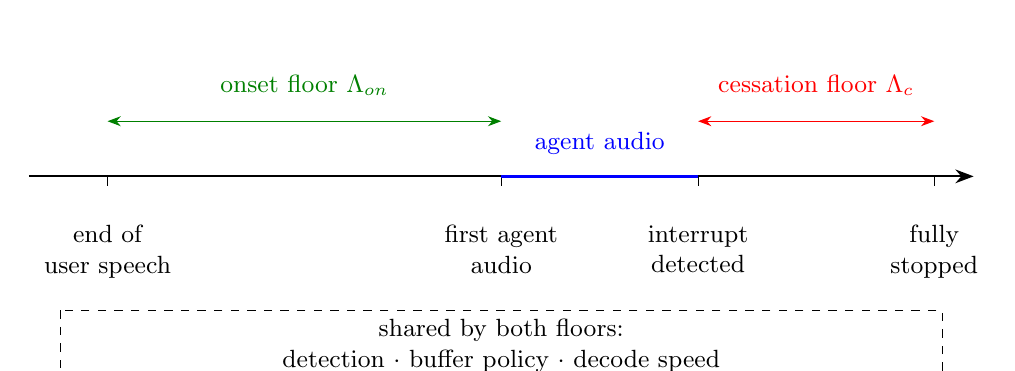
\begin{tikzpicture}[>=Stealth, font=\small]
  % Timeline axis
  \draw[thick,->] (0,0) -- (12,0);
  % Marks
  \draw (1,0) -- (1,-0.12); \node[below,align=center] at (1,-0.5) {end of \\ user speech};
  \draw (6,0) -- (6,-0.12); \node[below,align=center] at (6,-0.5) {first agent \\ audio};
  \draw (8.5,0) -- (8.5,-0.12); \node[below,align=center] at (8.5,-0.5) {interrupt \\ detected};
  \draw (11.5,0) -- (11.5,-0.12); \node[below,align=center] at (11.5,-0.5) {fully \\ stopped};
  % Agent audio bar
  \draw[very thick,blue] (6,0) -- (8.5,0);
  \node[blue,above] at (7.25,0.15) {agent audio};
  % Onset span
  \draw[<->,green!50!black] (1,0.7) -- (6,0.7);
  \node[green!50!black,above] at (3.5,0.9) {onset floor $\Lambda_{on}$};
  % Cessation span
  \draw[<->,red] (8.5,0.7) -- (11.5,0.7);
  \node[red,above] at (10,0.9) {cessation floor $\Lambda_c$};
  % Shared subsystems note (box sized to the two text lines)
  \draw[dashed] (0.4,-1.7) rectangle (11.6,-2.6);
  \node[align=center] at (6.0,-2.15) {shared by both floors:\\ detection $\cdot$ buffer policy $\cdot$ decode speed};
\end{tikzpicture}
%
\caption{The two responsiveness floors on a single turn timeline. Onset spans the detectable
end of user speech to first audible agent audio; cessation spans interruption onset to the end
of all in-flight audio. The detection, buffer, and decode subsystems are shared by both floors.
\label{fig:two_floors}}
\end{figure}

\begin{figure}[t]
\centering
% The three interruption phases and the react path each one takes.
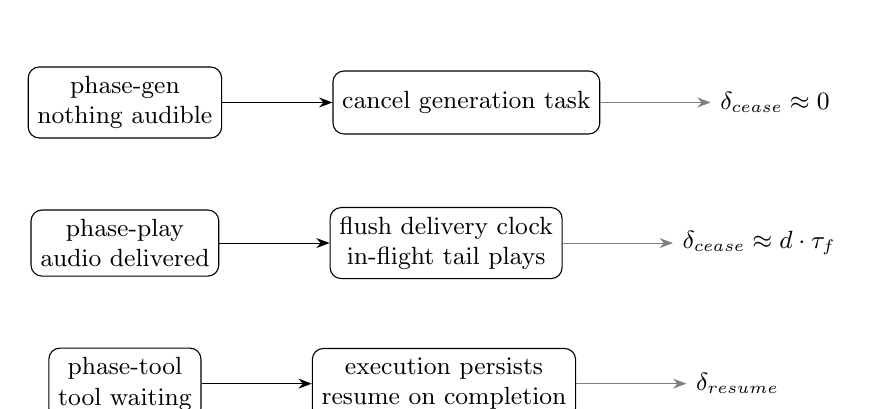
\begin{tikzpicture}[>=Stealth, font=\small, node distance=9mm and 14mm,
  box/.style={draw, rounded corners, align=center, minimum height=8mm}]
  % Phase 1
  \node[box] (pgen) {phase-gen\\nothing audible};
  \node[box, right=of pgen] (rg) {cancel generation task};
  \node[right=of rg] (og) {$\delta_{cease} \approx 0$};
  \draw[->] (pgen) -- (rg); \draw[->,gray] (rg) -- (og);
  % Phase 2
  \node[box, below=of pgen] (ppl) {phase-play\\audio delivered};
  \node[box, right=of ppl] (rpl) {flush delivery clock\\ in-flight tail plays};
  \node[right=of rpl] (opl) {$\delta_{cease} \approx d\cdot\tau_f$};
  \draw[->] (ppl) -- (rpl); \draw[->,gray] (rpl) -- (opl);
  % Phase 3
  \node[box, below=of ppl] (ptl) {phase-tool\\tool waiting};
  \node[box, right=of ptl] (rtl) {execution persists\\resume on completion};
  \node[right=of rtl] (otl) {$\delta_{resume}$};
  \draw[->] (ptl) -- (rtl); \draw[->,gray] (rtl) -- (otl);
\end{tikzpicture}
%
\caption{The three interruption phases and the react paths each one takes: phase-gen is
task-cancel, phase-play is delivery flush, phase-tool reduces to resumption after the
background tool completes.
\label{fig:interruption_phases}}
\end{figure}

\begin{figure}[t]
\centering
% Event algebra of the orchestrator: generic events, three clocks, reentry.
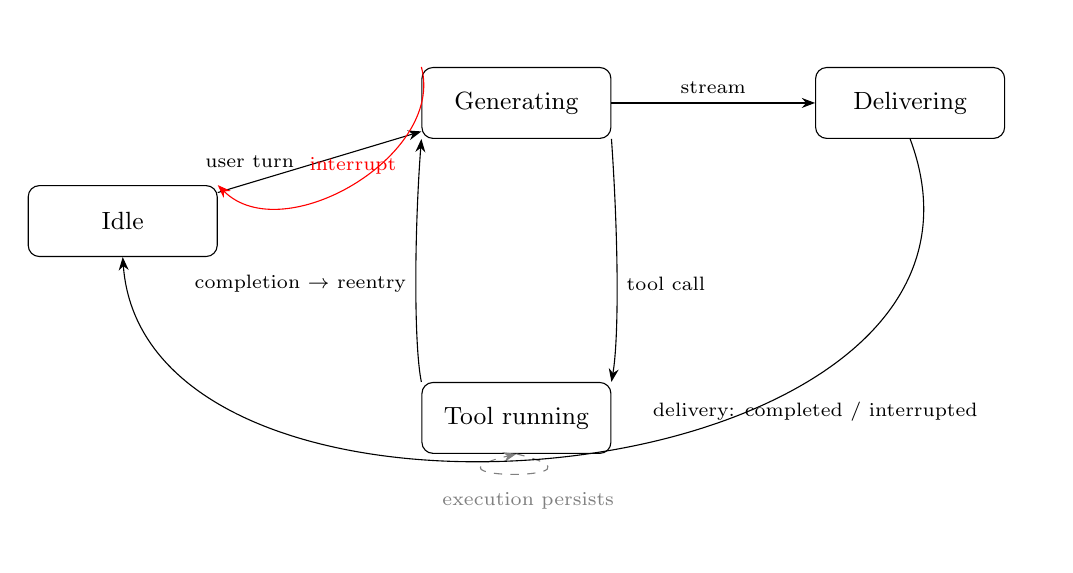
\begin{tikzpicture}[>=Stealth, font=\small,
  st/.style={draw, rounded corners, align=center, minimum height=9mm, minimum width=24mm},
  ev/.style={->,>=Stealth}]
  \node[st] (idle) at (0,0) {Idle};
  \node[st] (gen)  at (5,1.5) {Generating};
  \node[st] (del)  at (10,1.5) {Delivering};
  \node[st] (tool) at (5,-2.5) {Tool running};
  % user turn: idle -> generating (diagonal)
  \draw[ev] (idle) -- (gen) node[midway,above,font=\scriptsize,left=2mm]{user turn};
  % stream: generating -> delivering (straight, label above)
  \draw[ev] (gen) -- (del) node[midway,above,font=\scriptsize]{stream};
  % interrupt: red arc OVER the top left (cancels generation only, not tools)
  \draw[ev,red] (gen.north west) to[bend left=75]
    node[midway,above,font=\scriptsize,red]{interrupt} (idle.north east);
  % tool call: right bulge down from generation to the tool
  \draw[ev] (gen.south east) .. controls (6.3,-0.3) and (6.3,-1.5) .. (tool.north east)
    node[pos=0.5,right,font=\scriptsize]{tool call};
  % completion -> reentry: left bulge up from the tool to generation
  \draw[ev] (tool.north west) .. controls (3.7,-1.6) and (3.7,-0.2) .. (gen.south west)
    node[pos=0.5,left,font=\scriptsize]{completion $\rightarrow$ reentry};
  % tool execution persists across interruption (self-loop under the tool)
  \draw[dashed,->,gray] (tool.south) .. controls (6.4,-3.3) and (3.6,-3.3) .. (tool.south);
  \node[gray,font=\scriptsize] at (5.15,-3.55) {execution persists};
  % delivery outcomes: one outer loop around the right and bottom (clear of everything)
  \draw[ev] (del.south) .. controls (11.7,-3.5) and (0.3,-4.6) .. (idle.south)
    node[pos=0.30,below,font=\scriptsize,xshift=1.5mm,yshift=-1mm]{delivery: completed / interrupted};
\end{tikzpicture}
%
\caption{The event algebra of the orchestrator: user turns and tool completions are generic
events; delivery status reports playback; interruption cancels generation while the tool clock
persists and re-enters on completion.
\label{fig:event_loop}}
\end{figure}

\begin{figure}[t]
\centering
% Tool placement against the onset floor: only a serial type-A tool gates first audio;
% background dispatch, lead-in hiding, and background clocks all move off the floor.
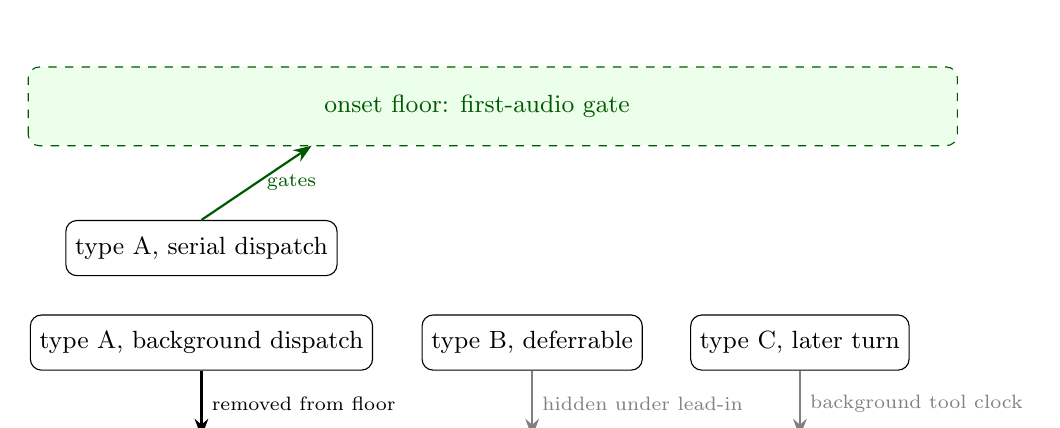
\begin{tikzpicture}[>=Stealth, font=\small, box/.style={draw, rounded corners,
  align=center, minimum height=7mm}]
  % Onset floor band (top, horizontal)
  \draw[fill=green!8, draw=green!35!black, dashed, rounded corners] (-2.2,3.2) rectangle (9.6,4.2);
  \node[green!35!black] at (3.5,3.7) {onset floor: first-audio gate};
  % Serial type A -> INTO the band (gates)
  \node[box] (as) at (0,1.9) {type A, serial dispatch};
  \draw[->,thick,green!35!black] (as.north) -- (1.4,3.2) node[midway,right,font=\scriptsize]{gates};
  % Type A background -> away (down)
  \node[box] (ab) at (0,0.7) {type A, background dispatch};
  \draw[->,thick] (ab.south) -- (0,-0.5) node[midway,right,font=\scriptsize]{removed from floor};
  % Type B -> away (down)
  \node[box] (bt) at (4.2,0.7) {type B, deferrable};
  \draw[->,thick,gray] (bt.south) -- (4.2,-0.5) node[midway,right,font=\scriptsize]{hidden under lead-in};
  % Type C -> away (down)
  \node[box] (ct) at (7.6,0.7) {type C, later turn};
  \draw[->,thick,gray] (ct.south) -- (7.6,-0.5) node[midway,right,font=\scriptsize]{background tool clock};
\end{tikzpicture}
%
\caption{Tool placement against the onset floor: a serial type-A tool gates first audio
(inside the band); background dispatch removes it from the floor (arrow away from the band);
type-B is hidden behind delivery lead-in and type-C behind the background tool clock.
Only the earliest genuinely audio-gating type-A result stays on the floor; for a parallel
DAG it is the critical path, not the sum.
\label{fig:tool_hiding}}
\end{figure}


\section{The Practical Question: Which Cascade Architecture?}
\label{sec:practical}
% §5 The Practical Question: Which Cascade Architecture?
Practitioners currently choose between four concrete cascade configurations for a realtime,
tool-using, long-session assistant:
a serial graph orchestrator (no decoupling, no filler),
the same with manual filler,
the same with model-uttered (LLM) filler, and
a decoupled, event-driven runtime with tools on a background clock.
The two-floor model assigns each configuration its onset and cessation behaviour in one table
(Table~\ref{tab:architectures}).

\begin{table}[t]
\centering
\begin{tabular}{p{0.30\textwidth}p{0.32\textwidth}p{0.30\textwidth}}
\toprule
\textbf{Architecture} & \textbf{Onset} & \textbf{Cessation} \\
\midrule
Serial graph (all clocks coupled) & pays reducible latency serially &
can cancel generation; checkpoint preserves state, but the coupled loop drags tool-waits and
delivery into the stop path \\
\midrule
Serial graph + manual filler & onset masked at delivery layer &
manual filler shortens the interruption tail: the classic barge-in-friendly device \\
\midrule
Serial graph + LLM filler & onset masked but fragment may bleed or duplicate in the committed
text & no cessation gain; unretractable filler corrupts delivered content per
Corollary~\ref{cor:filler} \\
\midrule
Event-driven, decoupled clocks & hides reducible latency during user speech &
owns both floors: generation-interruptible, execution-persistent, atomically committed batches
(Lemma~\ref{lem:serializability}) \\
\bottomrule
\end{tabular}
\caption{The four cascade architectures mapped onto the two-floor model. The event-driven row
is a sufficiency statement (Definitions~\ref{def:interruptibility} and~\ref{def:clocks}), not
an in-principle uniqueness claim: a graph orchestrator that hosts async nodes, background
dispatch, and checkpoint reentry can emulate it at expressiveness cost.
\label{tab:architectures}}
\end{table}

Two consequences follow.
First, for single-hop turns there is no reducible latency to hide and no tail to manage: under
a fixed in-flight policy all four configurations meet the same floor, so orchestration choice
is noise.
Second, for tool and long-duration turns the configurations separate sharply: tool round-trips
land on the onset floor unless dispatched to a background clock
(Theorem~\ref{thm:tool_hiding}), and interruption behaviour is governed by the delivery tail
(Theorem~\ref{thm:cessation_floor}).
This separation is the pattern that tool-agent latency evaluations reveal: they measure
accuracy and liveness jointly but do not predict liveness from tool-DAG structure
\citep{taubench2024}, whereas our model predicts exactly the turns where structure dominates.
An assistant that mostly answers from memory can stay on a serial graph with manual filler;
an assistant whose turns habitually touch the bank, the card service, or multi-step skills
needs the decoupled runtime to avoid paying each tool round-trip inside the user's perceived
silence.


\section{Open Problems}
\label{sec:open_problems}
% §6 Open Problems
The two-floor model leaves deliberately open problems that we list with their intended next
steps.

\paragraph{Standardised cessation and perceived-V2V measurement.}
Industry measures barge-in timing ad hoc; there is no shared definition and no protocol for the
perceived variant (audio actually reaching the speaker, including transport and devices).
A standardised protocol for \emph{perceived} response onset and cessation -- analogous to the
reporting standards that exist for static benchmarks -- would let the floors of
Theorem~\ref{thm:cessation_floor} be compared across systems and labs.
Our smoke anchor is an approximation; the protocol is the full measurement campaign.

\paragraph{Guardrail re-arming under reentry.}
An execution-persistent orchestrator re-enters the model on every tool completion.
Each re-entry is a fresh generation window and therefore a fresh place a guardrail must arm
\citep{dong2024building}.
The safety-deadline question -- where a guardrail can sit inside the floor without inflating it
-- becomes a per-reentry schedulability problem with the same shared-dependency structure as
Proposition~\ref{prop:floor_dependency}.
This connects the present paper to the open streaming-safe guardrail gap and its
linear-cost certification question.

\paragraph{Forgetting and context compaction across long sessions.}
Long stateful sessions grow the prefill contribution to the onset floor over time.
Managing what the agent retains -- compaction, eviction, external memory -- is a
\emph{deadline-aware} policy in the same sense as buffer depth is here
\citep{xiao2023streamingllm,packer2023memgpt}.
A ``forgetting floor'' that ties retained context to the onset budget is the natural companion
result.

\paragraph{Cancellable vs irrevo\-cable tools.}
The ``tool persistence under cancellation is safe'' headline of
Section~\ref{sec:analysis} is \emph{protocol}-safe: it guarantees a provider-valid history
(Lemma~\ref{lem:serializability}).
It is not automatically \emph{business}-safe.
For irrevocable, side-effecting tools -- payment, transfer, authorization -- a resumed context
that re-runs the same tool risks double-execution or double-charge.
Idempotency keys, revocation, and explicit re-authorisation are therefore prerequisites for
persisting business-critical tools across an interruption.
This is a separate concern from the type A/B/C classification: tool typing describes when
a result is needed for audio, not whether re-running the persisted call is safe.

\paragraph{Learned turn-end prediction.}
Reacting to an interruption is the worst case; predicting it is the improvement.
The companion paper's predictive-stop ceiling and this paper's reactive floor delimit the
intervention window, and learning to shrink it is an open empirical question.

\paragraph{Predictive dispatch across tool types.}
Reclassifying a tool from type A to type B at runtime -- dispatching it off a partial
transcript before the turn is final -- is the engine behind deployed pre-EOU dispatch and
prefetch systems \citep{specrag2024,agentsnotenough2024,lin2026fdbv3}.
A composition rule that states when such pre-dispatch is safe, and what it costs in accuracy,
remains open.


\section{Discussion}
\label{sec:discussion}
% §7 Discussion
We are explicit about what this paper does and does not claim.

\paragraph{Scope of the evidence.}
The formal results are the contribution; the orchestrator PoC verifies the \emph{semantics}
the results assume, and the smoke anchor instantiates the quantities on a simulated delivery
clock.
There is no real ASR, TTS, or language model in the loop, and the frame and tool latencies are
synthetic.
The anchor is therefore a feasibility instance with arbitrary units, not a benchmark.
The per-architecture cessation values a production system would observe also depend on its
specific synthesis queueing and its backend tool latency, which real deployment telemetry
confirms can reach $\sim$1~s per round trip.

\paragraph{No uniqueness claim.}
The event-driven configuration is presented as a \emph{sufficient}, idiomatic way to own both
floors (Definitions~\ref{def:clocks} and~\ref{def:interruptibility}).
Serial topologies can host async nodes, background dispatch, and checkpoint reentry and thereby
emulate the same capability; the paper's claim is about idiomatic expressiveness, not
in-principle precedence.
Similarly, Proposition~\ref{prop:floor_dependency} is a dependency statement under a fixed in-flight
policy, not a claim that the floors are independent in general.

\paragraph{Policy vs physics.}
Theorem~\ref{thm:cessation_floor} separates \emph{can stop} from \emph{should stop}.
Ceasing fast is not always the right user experience, and an engagement-aware policy may
legitimately decide to keep the floor \citep{bohus2011interruptions}.
The floor is a capability bound, and the paper makes no claim about optimising raw cession speed
in every turn.

\paragraph{Relation to product vocabulary.}
The onset side maps one-to-one onto the server-side voice-to-voice metric used in deployment --
the interval from detected end of user speech to first audio leaving the synthesis server.
This paper adds the symmetrical interval on the other side of an interruption, which
production telemetry today does not emit at all.
Of the two, cessation is the one most frequently felt on tool-heavy turns and the one with no
standard definition, reinforcing the motivation of Section~\ref{sec:introduction}.

\paragraph{Citation status.}
Related-work references were verified against the arXiv API and Crossref on 2026-09-01,
including a 2025--26 sweep that surfaced the full-duplex and interruption benchmarks cited
in Section~\ref{sec:background}.
The companion onset-floor paper is available as an alphaXiv preprint
(alphaXiv:2608.latency-floor-cascade-voice-agents); the formal results of
Section~\ref{sec:analysis} do not depend on its indexing status.

\paragraph{Relation to the companion paper.}
Where the companion paper \citep{latencyfloor2025} bounded response onset from outside the stage, this paper bounds
response cessation from inside it, and reuses the same reducible/irreducible intuition and the
same $200$~ms perceptual anchor.
Together the two papers give a two-sided picture of realtime responsiveness for cascade
agents.


\section{Conclusion}
\label{sec:conclusion}
% §8 Conclusion
Real-time responsiveness in cascade voice agents is two-sided, and this paper supplies the side
that has neither a standard definition nor a bound: the cessation floor.
We close the gap with a two-floor model and a phase-conditioned result: cessation grows with
in-flight audio up to the committed buffer depth, generation cancellation is prompt and
independent of the delivery tail, and resumption after interruption is dominated by tool
round-trip cost unless tools run on a background clock.

The enabling mechanism is orchestration, not any single component.
Decoupling generation, delivery, and tool clocks makes an agent generation-interruptible and
execution-persistent at once, and an API-serializability lemma guarantees that cancelling
generation never strands a pending tool batch.
A small, tested orchestrator verifies the semantics, and a monotonic-clock smoke anchor
instantiates the quantitative shape: cessation linear in in-flight audio, prompt
depth-independent cancellation, and tool-dominated resumption.

The practical conclusion answers the debate that motivated this work.
For an assistant whose turns are short and memory-bound, orchestration choice is noise under a
fixed in-flight policy.
For an assistant whose turns routinely call tools -- a bank, a card service, a multi-step
skill -- an idiomatically decoupled runtime avoids paying each round trip inside the
user's perceived silence and manages the interruption tail.
Framework arguments settle no data; the two floors settle the question: onset and cessation
together describe perceived responsiveness, and the onset guarantee now extends to the
orchestration that schedules reasoning, tools, and interruptions.


\bibliographystyle{plainnat}
\bibliography{main}

\end{document}
